\section{Experiments}
\label{sect:experiments}

We now perform evaluation and the comparison of the two approaches and their variants. 

\bigskip\indent\textbf{Datasets and protocols} 

\label{sect:datasets}
\bigskip\indent\textbf{Surveillance data}\\
\label{sect:surveillance}
For the surveillance image domain ($A$, as denoted in \sect{strategies}), we have obtained a surveillance dataset comprising faces from five cameras in Moscow subway. Our dataset consists of two subsets of images, denoted as \texttt{LR} (low-resolution) and \texttt{HR} (high-resolution) according to their size in pixels. Sizes are calculated as the face bounding box heights. Mean face heights for \texttt{LR} and \texttt{HR} subsets were $49.72$ and $106.19$ pixels correspondingly. The \texttt{LR} images range from $37$ to $63$ pixels, and \texttt{HR} images from $75$ to $224$. The DLib \citep{dlib09} library was used for face detection and subsequent alignment. 
 
Generally, the identities of people occurring in the video are unknown, and therefore we mine matching faces in the dataset by considering temporal tracks in videos. We assume that face images from different tracks are non-matching. The matching pairs then correspond to pairs of faces from the same track, such that one image belongs to the LR subset and the other belongs to the HR subset. Columns 1 and 3 in \fig{lr_hr_gan_res_ytube_initial_degraded} show some examples of matched pairs. Usually, the quality of face images increases when the person approaches the camera, and therefore \texttt{HR}-subset images are often (but not always) visually better than those present in the \texttt{LR} subset. The division into \texttt{LR} and \texttt{HR} subsets is introduced to ensure that the matched pairs of frames correspond to distinct frames of the temporal tracks. We stress that the mined matching pairs are used for evaluation (testing) only and are not used for training of any networks in our experiments.

We use $96$ identities that are present in both \texttt{LR} and \texttt{HR} for parameter validation and $279$ identities for test. For each of the test identity, there is a pair of matching tracks (one LR track and one HR track). The goal of algorithms is then to build descriptors that would be similar for frames coming from the HR and the LR tracks of the same identity, and would be dissimilar for the HR and the LR tracks corresponding to different identities. Overall, $3,891$ images were used for test.

$4,979$ images of identities not present in the test set are used for training the unsupervised domain transfer described in \sect{domain_transfer} (tracking-based information was not used to train the ConvNets). The mean number of frames for each identity in \texttt{LR} and \texttt{HR} test data are $18.62$ and $17.72$ correspondingly.
 
 
  To evaluate the recognition quality, we match identities across the \texttt{LR} and \texttt{HR} in the following way: we calculate the cosine similarity between the frame set $t_{id_1}^{LR}$ of identity $id_1$ and the frame set, $t_{id_2}^{HR}$ of identity $id_2$ by averaging the similarities of each pair of frames: 

 \begin{align}
     S \left(t_{id_1}^{LR},t_{id_2}^{HR}\right) = \frac {1} { |t_{id_1}^{LR}|*|t_{id_2}^{HR}|}\sum_{i=0, j= 0}^{|t_{id_1}^{LR}|, |t_{id_2}^{HR}|} S \left(f_{id_1,i}^{LR},f_{id_2,j}^{LR} \right), \\
     S\left((f_{id_1,i}^{LR},f_{id_2,j}^{LR}\right) =  cos\left(d_{id_1,i}^{LR},d_{id_2,j}^{LR}\right),
 \end{align}
 where $d_{id_1,i}^{LR}$,$d_{id_2,j}^{HR}$ are the descriptors of the corresponding frames calculated by face recognition neural network $R$ \ref{sect:face_recognition}.
%f_{id_1,i}^{low} \subseteq t_{id_1}^{low} , %f_{id_2,j}^{low} \subseteq t_{id_1}^{low}

% To evaluate the recognition quality, we match identities across the \texttt{LR} and \texttt{HR} in the following way: we calculate the cosine similarity between the frame set $t_{id_1}^{LR}$ of identity $id_1$ and the frame set, $t_{id_2}^{HR}$ of identity $id_2$ by averaging the similarities of each pair of frames: 

% \begin{align}
%     S(t_{id_1}^{LR},t_{id_2}^{HR}) = \sum_{i=0, j= 0}^{|t_{id_1}^{LR}|, |t_{id_2}^{HR}|} S(f_{id_1,i}^{LR},f_{id_2,j}^{LR} ), \\
%     S(f_{id_1,i}^{LR},f_{id_2,j}^{LR} ) =  cos(d_{id_1,i}^{LR},d_{id_2,j}^{LR}),
% \end{align}
% where $d_{id_1,i}^{LR}$,$d_{id_2,j}^{HR}$ are the descriptors of the corresponding frames calculated by face recognition neural network $R$ \ref{sect:face_recognition}.
%f_{id_1,i}^{low} \subseteq t_{id_1}^{low} , f_{id_2,j}^{low} \subseteq t_{id_1}^{low}

\bigskip\indent\textbf{Evaluation metrics}\\

We focus our evaluation on the surveillance data domain. As already mentioned above, during evaluation, we compare pairs of \textit{tracks}, where the first track comes from the \texttt{LR} subset and the second track comes from the \texttt{HR} subset. 

When comparing the two tracks using the recognition metrics, we match all possible pairs of frames and compute the mean average cosine similarity between the computed descriptors over all pairs (more sophisticated schemes involving minimal pairs did not result in better performance). Depending on whether the mean average cosine similarity is higher or lower than a certain threshold $\tau$, we treat a certain pair of tracks as matching or non-matching.

By considering various $\tau$, we then compute the \textit{ROC curve}, the area under the ROC curve (ROC AUC), the $100$\% - EER (Equal Error Rate) statistics, and the average precision (AP) metrics. 



\bigskip\indent\textbf{Internet data}\\
For the Internet image domain ($B$, as denoted in \sect{strategies}) we use three face recognition datasets: Celeb-A \citep{liu2015faceattributes}, YouTube Faces (YTF) \citep{WolfHM11} and the VGG Face datasets \citep{parkhi2015deep}.

The Celeb-A dataset~\citep{liu2015faceattributes} consists of $202,599$ images of high quality and is used for training CycleGAN-based  domain transfer described in \sect{domain_transfer}. 

The Youtube Faces (YTF) dataset~\citep{WolfHM11} and the VGG Face dataset~\citep{parkhi2015deep} are used for the finetuning of the face recognition neural network as described in \sect{face_recognition}. YTF consists of $3,425$ videos of $1,595$
people collected from YouTube, with an average of 2 videos per identity. The VGG Face dataset contains $2,6$M images of $2,622$ identities. We show that face recognition improves, when using our CycleGAN-based data augmentation when trained on either YTF or VGG Face. Generally, YTF and VGG Face represent two different types of face images that can be mined from the Internet (with YTF having lower quality).





%All the images in the four mentioned datasets are aligned in the same way: DLib is used for feature detection and alignment by $3$ eyes and nose feature-points, so that their target positions are the following :



\bigskip\indent\textbf{Compared variants of recognition networks}\\
\label{sect:ft}
We compare the following adaptation/transfer strategies for training the recognition networks:
\begin{itemize}

\item \textit{no ft} -- the pre-trained VGG-face model~\citep{parkhi2015deep} with no re-training is used to compute descriptors of the surveillance-domain images.


\item \textit{ft initial} -- the VGG-face model is fine-tuned using the original version of the YTF or the VGG Face datasets (no domain adaptation). 

\item \textit{ft degraded} -- the VGG-face model fine-tuned using the degraded version of the YTF or VGG Face datasets transferred to the target (surveillance) domain (using domain adaptation),

\item \textit{ft union} -- the VGG-face model fine-tuned using \textbf{both} the initial and the degraded versions  of the YTF or VGG Face datasets (using domain adaptation). 

\end{itemize}

The YTF dataset images and the corresponding degraded images are shown  in \fig{lr_hr_gan_res_ytube_initial_degraded} (the two last columns).
%The two last variants \textit{ft degraded} and \textit{ft union} perform domain adaptation, as all or part of the training data are transferred to the target domain.



 
\bigskip\indent\textbf{Training details}\\
\label{sect:training}
The CycleGAN-based domain transfer consists of $3$ types of modules (see \sect{domain_transfer}).
Encoders $E_A$ and $E_B$ have the following architecture:
\begin{center}
\begin{scriptsize}
\begin{tabular}{l | c c c c c c c}
\hline
  \#conv layer      &1   &2      &3    &4     &5    &6    &7     \\
  num of filters    &32  &64     &128  &128   &128  &128  & 128  \\
  kernel size       &3   &3      &3    &3     & 3   &3    &3     \\
  stride/pad        &1/0 &2/1    &2/1  &1/1   &1/1  &1/1  & 1/1  \\
  \#res block       & -  & -     & -   & 0    &0    &1    &1     \\
\hline
\end{tabular}
\end{scriptsize}
\end{center}
\vspace{0.5em}

% EncShared(
%   (from_img): ModuleList(
%     (0): Conv2d(3, 32, kernel_size=(1, 1), stride=(1, 1))
%   )
%   (enc_blocks): ModuleList(
%     (0): Sequential(
%       (0): Conv2d(32, 64, kernel_size=(3, 3), stride=(2, 2), padding=(1, 1), bias=False)
%       (1): InstanceNorm2d(64, eps=1e-05, momentum=0.99, affine=True)
%       (2): LeakyReLU(0.01, inplace)
%     )
%     (1): Sequential(
%       (0): Conv2d(64, 128, kernel_size=(3, 3), stride=(2, 2), padding=(1, 1), bias=False)
%       (1): InstanceNorm2d(128, eps=1e-05, momentum=0.99, affine=True)
%       (2): LeakyReLU(0.01, inplace)
%     )
%   )
% )

% Enc(
%   (enc_blocks): ModuleList(
%   )
%   (res_blocks): ModuleList(
%     (0): ResBlock(
%       (model): Sequential(
%         (0): Conv2d(128, 128, kernel_size=(3, 3), stride=(1, 1), padding=(1, 1), bias=False)
%         (1): InstanceNorm2d(128, eps=1e-05, momentum=0.99, affine=True)
%         (2): LeakyReLU(0.01, inplace)
%         (3): Conv2d(128, 128, kernel_size=(3, 3), stride=(1, 1), padding=(1, 1), bias=False)
%         (4): InstanceNorm2d(128, eps=1e-05, momentum=0.99, affine=True)
%       )
%     )
%     (1): ResBlock(
%       (model): Sequential(
%         (0): Conv2d(128, 128, kernel_size=(3, 3), stride=(1, 1), padding=(1, 1), bias=False)
%         (1): InstanceNorm2d(128, eps=1e-05, momentum=0.99, affine=True)
%         (2): LeakyReLU(0.01, inplace)
%         (3): Conv2d(128, 128, kernel_size=(3, 3), stride=(1, 1), padding=(1, 1), bias=False)
%         (4): InstanceNorm2d(128, eps=1e-05, momentum=0.99, affine=True)
%       )
%     )
%   )
% )

The architecture of generators $G_A$, $G_B$ is as follows:
\begin{center}
\begin{scriptsize}
\begin{tabular}{l | c c c c c c c}
\hline
  \#conv layer      &1      &2    &3     &4    &5    &6    & 7 \\
  num of filters    &128    &128  &128   &128  &64   &32   & 3 \\
  kernel size       &3      &3    &3     & 3   &3    &3    & 1 \\
  stride/pad        &1/1    &1/1  &1/1   &1/1  &1/1  &1/1  & 1/0  \\
  \#res block       &0      &0    &1     &1    &-    &-    & -  \\
\hline
\end{tabular}
\end{scriptsize}
\end{center}
\vspace{0.5em}

Instance normalization~\citep{UlyanovVL17} and Leaky ReLU~\citep{HeZRS15} with negative slope set to $0.01$ are inserted after each of the convolution layers. Except for the last layers of $G_A$ and $G_B$, where \texttt{tanh} non-linearity is used (for the subsequent feeding of the result into the discriminator). To keep the input image size unchanged,  $\times 2$ nearest neighbor upsampling is done before the convolutions $3$ and $4$.
All input images are normalized to $64\times64$ pixels (output images are therefore of the same size). 


% Dec(
%   (to_img): ModuleList(
%     (0): Sequential(
%       (0): Conv2d(32, 3, kernel_size=(1, 1), stride=(1, 1))
%       (1): Tanh()
%     )
%   )
%   (upsample): Upsample(scale_factor=2, mode=nearest)
%   (res_blocks): ModuleList(
%     (0): ResBlock(
%       (model): Sequential(
%         (0): Conv2d(128, 128, kernel_size=(3, 3), stride=(1, 1), padding=(1, 1), bias=False)
%         (1): InstanceNorm2d(128, eps=1e-05, momentum=0.99, affine=True)
%         (2): LeakyReLU(0.01, inplace)
%         (3): Conv2d(128, 128, kernel_size=(3, 3), stride=(1, 1), padding=(1, 1), bias=False)
%         (4): InstanceNorm2d(128, eps=1e-05, momentum=0.99, affine=True)
%       )
%     )
%     (1): ResBlock(
%       (model): Sequential(
%         (0): Conv2d(128, 128, kernel_size=(3, 3), stride=(1, 1), padding=(1, 1), bias=False)
%         (1): InstanceNorm2d(128, eps=1e-05, momentum=0.99, affine=True)
%         (2): LeakyReLU(0.01, inplace)
%         (3): Conv2d(128, 128, kernel_size=(3, 3), stride=(1, 1), padding=(1, 1), bias=False)
%         (4): InstanceNorm2d(128, eps=1e-05, momentum=0.99, affine=True)
%       )
%     )
%   )
%   (dec_blocks): ModuleList(
%     (0): Sequential(
%       (0): Conv2d(128, 64, kernel_size=(3, 3), stride=(1, 1), padding=(1, 1))
%       (1): LeakyReLU(0.01, inplace)
%     )
%     (1): Sequential(
%       (0): Conv2d(64, 32, kernel_size=(3, 3), stride=(1, 1), padding=(1, 1))
%       (1): LeakyReLU(0.01, inplace)
%     )
%   )
% )


%Finally, discriminators $D_A$ and $D_B$ were derived from the
%VGG-face model~\citep{parkhi2015deep}, which was used for calculating face descriptors, leading to the following archiecture:
Finally, discriminators $D_A$ and $D_B$ have the following architecture: 
\begin{center}
\begin{scriptsize}
\begin{tabular}{l |c c c c c }
\hline
  \#conv layer      &1      &2    &3     &4    &5  \\
  num of filters    &64     &128  &256   &256  &1  \\
  kernel size       &3      &3    &3     & 3   &3  \\
  stride/pad        &2/1    &2/1  &2/1   &2/1  &1/0\\
\hline
\end{tabular}
\end{scriptsize}
\end{center}
\vspace{0.5em}
Leaky ReLU \citep{HeZRS15} with negative slope parameter set to $0.01$ is used as an activation. The final fully-connected layer with one output unit is added to $D_A$ and $D_B$.


% Dis(
%   (to_pred): ModuleList(
%     (0): Conv2d(256, 1, kernel_size=(1, 1), stride=(1, 1))
%     (1): Conv2d(256, 1, kernel_size=(1, 1), stride=(1, 1))
%   )
%   (blocks): ModuleList(
%     (0): Sequential(
%       (0): Conv2d(128, 256, kernel_size=(3, 3), stride=(2, 2), padding=(1, 1))
%       (1): LeakyReLU(0.01, inplace)
%     )
%     (1): Sequential(
%       (0): Conv2d(256, 256, kernel_size=(3, 3), stride=(2, 2), padding=(1, 1))
%       (1): LeakyReLU(0.01, inplace)
%     )
%   )
% )


According to the strategies described in \sect{ft}, we fine-tune the VGG-face model, having added new $128$-dimensional embedding layer instead of the initial classification layer (\textit{fc8}). All the results are reported for the \textit{fc7} layer though, as we found it to work better across all compared methods.

ADAM optimization~\citep{Kingma14} was used for both optimization objectives of the domain transfer task and the face recognition task, the learning rates were set to $1e-4$ and $1e-7$ correspondingly. Batch sizes were $16$ and $64$. Learning processes took $50$ epochs for the domain transfer,  and from $80$ to $200$ epochs for the face recognition task. Parameters $\lambda_1$ and $\lambda_2$ were set to $10$ in the loss \eq{domain_loss}. Parameters $\alpha$, $\beta$ and $C$ of the loss \eq{bindev} were set to $2$, $0.5$ and $10$.

For training the face recognition models described in \sect{ft}, the training batches had the following structure: in each batch, there were up to $3$ examples for each class for the VGG Face dataset and up to $10$ examples for the YTF dataset. For the \textit{ft union} model, each training batch was formed out of the examples of one of the domains. The sampling process alternated between the domains at each iteration.


  
   \begin{figure}
  \centering
    \includegraphics[width=\linewidth]{Chapters/facev1/Fig4.eps}
    \caption{The ROC curves for our face recognition models for different types of test data. Left -- \textit{no ft} model, test data transformation (the curve is denoted by 'restored') improves recognition. Middle -- \textit{ft initial}, the results for test data transformation are not clearly better than the results for initial images. Right -- \textit{ft union} model, the best results are for initial test data, without transformation. See \ref{sect:restoration_comparison} for the details. }\label{fig:roc_oxford_gan_vs_initial}
  \end{figure}

\newpage
\bigskip\indent\textbf{Does the translation to the Internet domain help recognition?} 
\label{sect:restoration_comparison}

We start by assessing the improvement that the restoration process brings to the recognition. For this we evaluate the performance of the three different recognition networks discussed above, when they are applied either to untransformed surveillance-domain images or to surveillance-domain images transformed to the Internet image domain (using the learned mapping $F^{A \rightarrow B}$). See  \fig{lr_hr_gan_res_ytube_initial_degraded} for the example results of the Internet domain  transfer.

The ROC-curves in  \fig{roc_oxford_gan_vs_initial} shows that while the restoration process helps for the \textit{no ft} network, it actually \textit{hurts} for the better-performing \textit{ft union} network. While trying to improve the results of the reverse transfer, we have also tried to transfer only the LR subset of the training images, while keeping the HR subset intact, but this lead to uniformly worse results.

We conclude that restoration does not necessarily help the recognition process in our setting. 

In the course of our experiments, we have also tried several different options for training CycleGAN. For example, we observed that the CycleGAN training scheme from \citep{ZhuPIE17} did not lead to visually good results for our data. Second, for the CycleGAN version mentioned in the paper, we have also tried an approach similar to that of \citep{sungatullina2018image}. In more details, we not only fed images to the higher-quality domain discriminator  $D^{I}$, but also intermediate features extracted from a pretrained face recognition network. As a result, we observed that ‘restoration’ transfer gave very visually plausible results, but recognition quality after such transform dropped considerably and was uniformly worse than all the results in \fig{roc_oxford_gan_vs_initial}. This might be due to non identity-preserving way of facial features change.


% \begin{figure}
%  \centering
%     \includegraphics[width=\linewidth]{Fig4.eps}
%     \caption{The change of the recognition metrics for our surveillance validation set. \textit{ft degraded} and \textit{ft union} models that use our image-level domain adaptation overfit less than \textit{ft initial} that use only the initial Internet-domain data. The improvement is consistent across the two cases when VGG face and YTF datasets were used as Internet image data. See section \ref{sect:ft} for the models description.}\label{fig:validation_ytube}
%   \end{figure}
  
  \begin{figure}

  \centering
    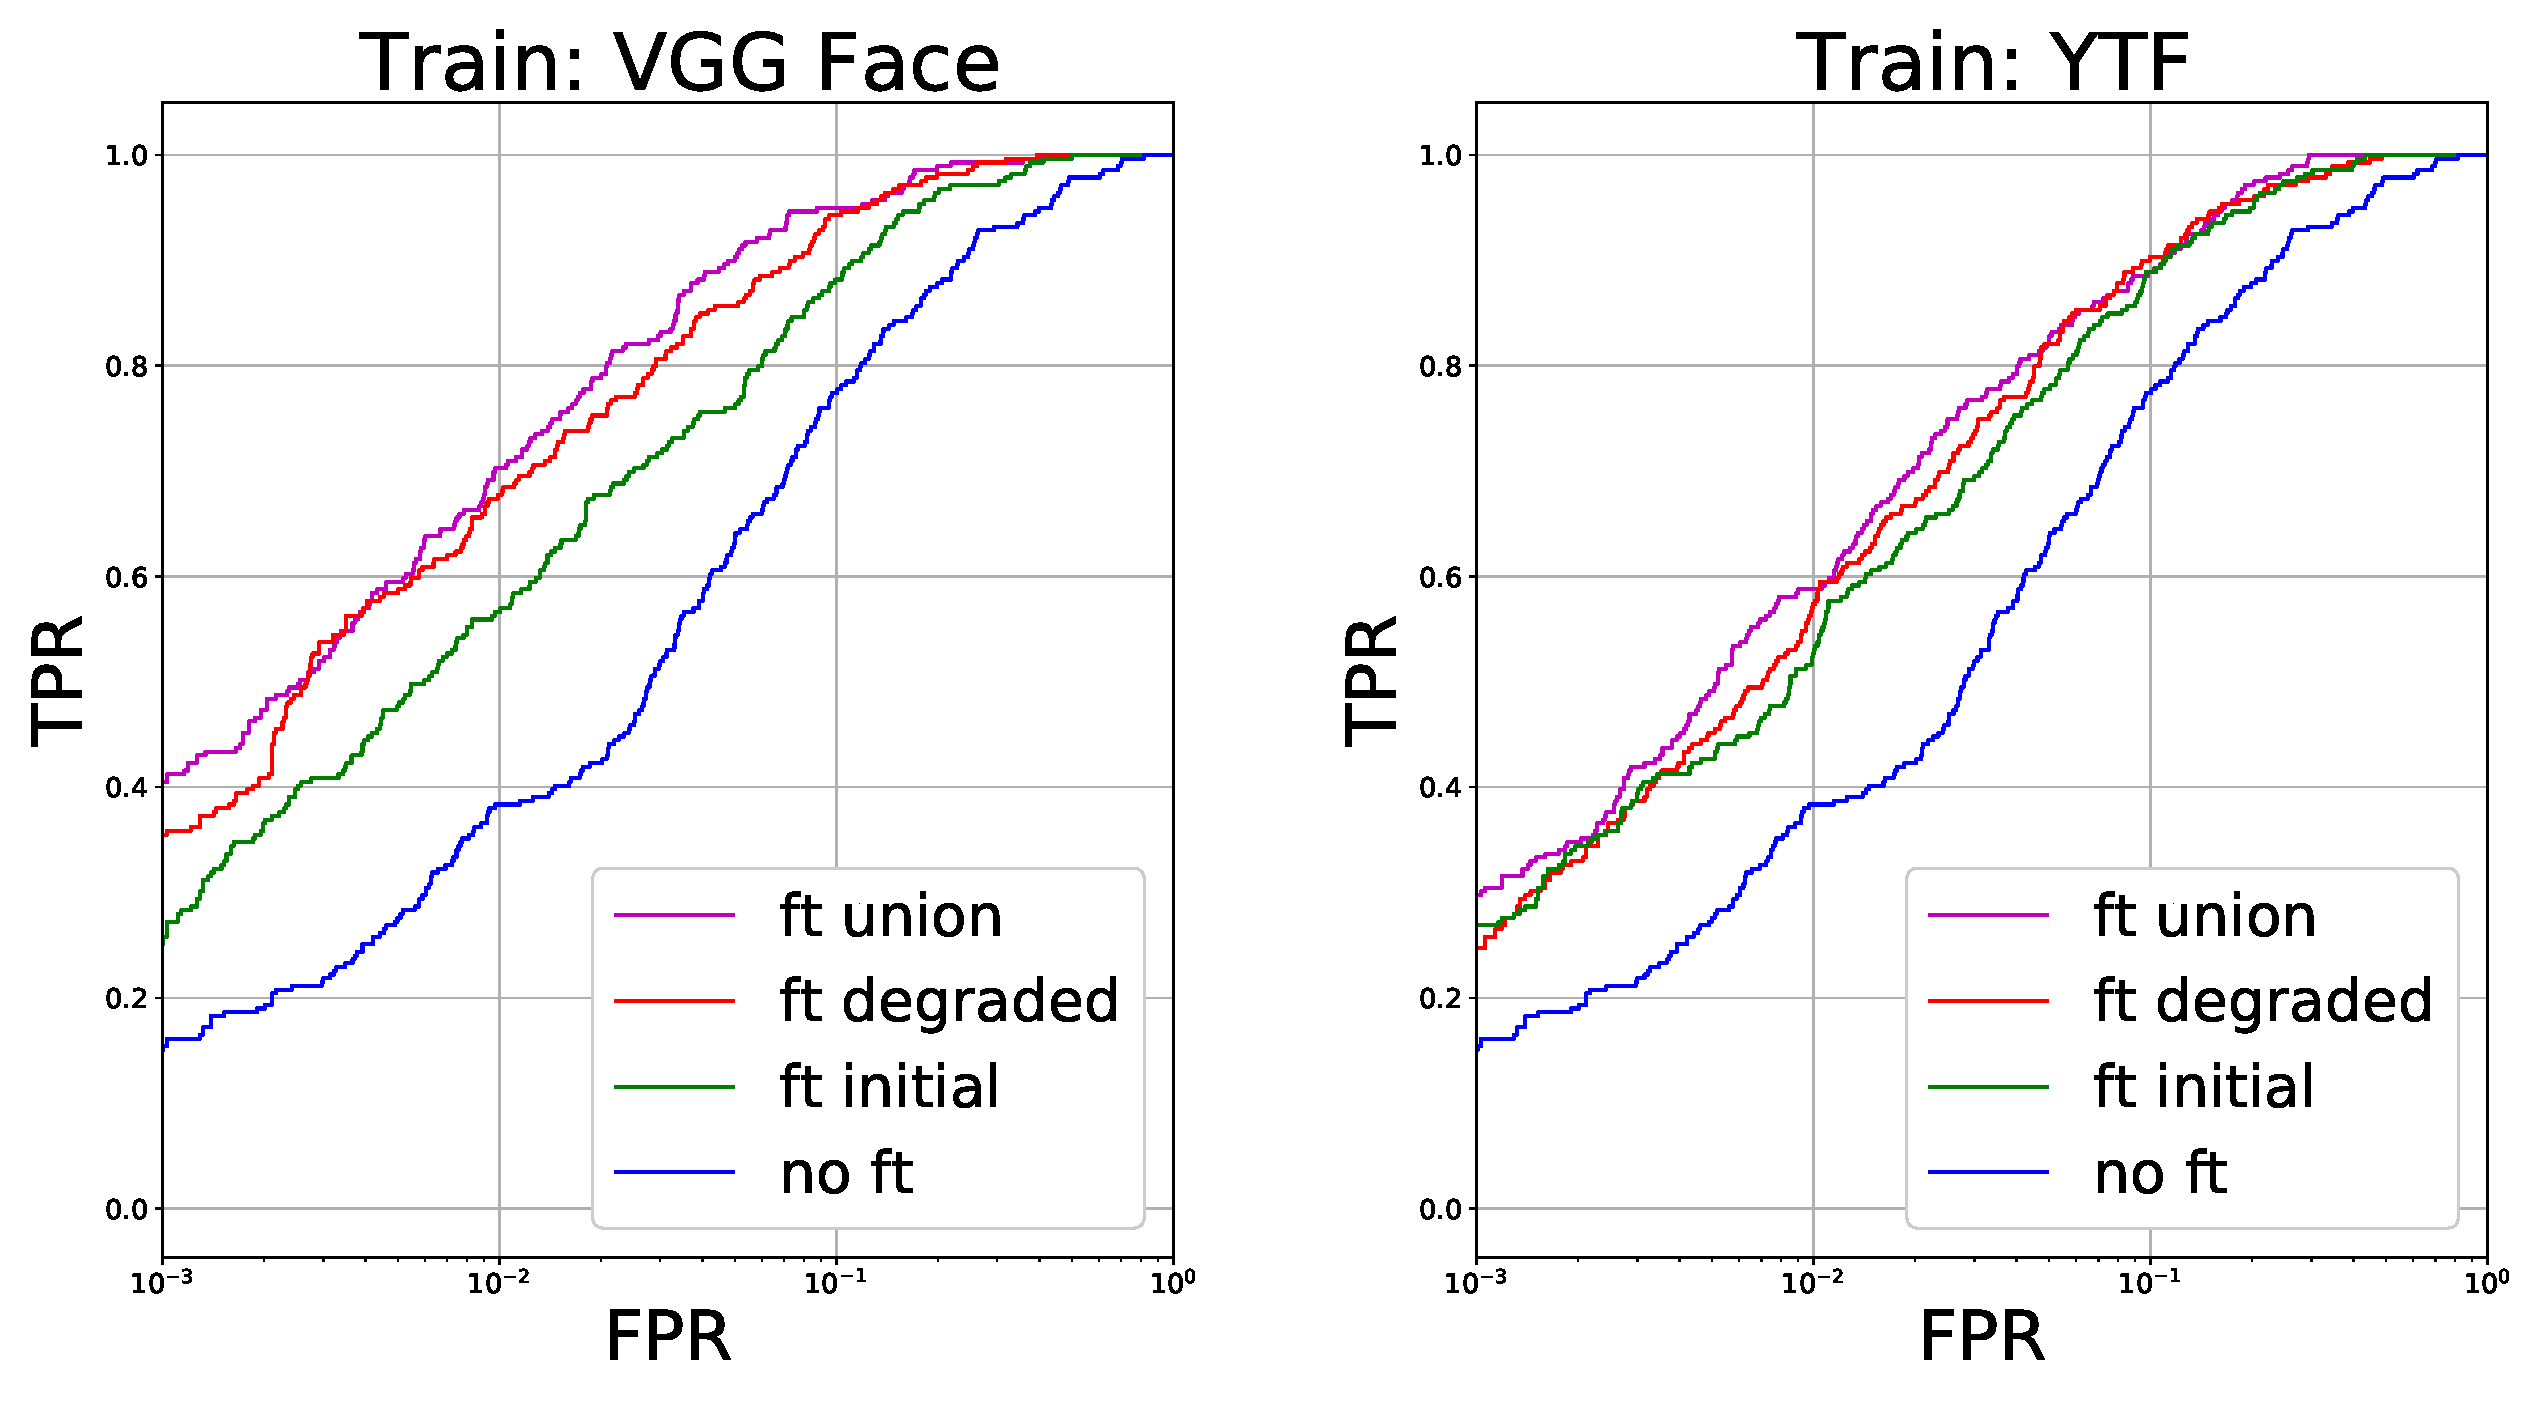
\includegraphics[width=\linewidth]{Chapters/facev1/Fig5.eps}
    \caption{The ROC curves for the fine-tuning strategies described in \sect{ft}. Our surveillance data is used for test. \textit{ft degraded} and \textit{ft union} models that use our image-level domain adaptation are better than other models. }\label{fig:roc_oxford_ytube}
  \end{figure}
  
 
\begin{table}
\centering
\flushbottom

\centering
\caption{Quality metrics for different face recognition models compared in this work (\ref{sect:ft}). Surveillance data are used for evaluation. The best model is \textit{ft union}, it is trained on both initial and degraded data.}
\label{tab:comparison}
\resizebox{0.7\columnwidth}{!}{
\begin{tabular}{c|ccc|ccc}
\hline
%\multicolumn{1}{|l|}{}   & \multicolumn{6}{c|}{Train datasets}                      \\ \hline
\multicolumn{1}{l|}{}   & \multicolumn{3}{c|}{train: VGG Face} & \multicolumn{3}{c}{train: YTF} \\ \hline
Fine-tuning type & 100\%$-$eer & roc auc & AP & 100\%$-$eer   & roc auc   & AP  \\ \hline
no ft                   &  83.89 & 91.86 & 22.04  &  83.89 & 91.86 & 22.04  \\ %\hline
ft initial               &  89.12 & 96.25 & 42.02  &  89.24 & 96.19 & 40.81 \\ %\hline
ft degraded             &  91.55 & 97.70 & 52.55 &  \bf{90.04} & 96.54 & 42.07   \\ %\hline
ft union                & \bf{92.94} &  \bf{98.08} & \bf{57.30}  &  89.37 & \bf{96.96} & \bf{45.45}      \\ \hline
\end{tabular}
}
\end{table}

  
  \begin{table}
\centering
\caption{Quality metrics of our approach compared to that of \citep{ganin2016domain} and \citep{SohnLZY0C17} and some combinations of these methods with ours. Surveillance data are used for evaluation. 'fm loss' and 'fr loss' stand for Feature Matching loss and Feature Reconstruction loss as defined in \citep{SohnLZY0C17}. 'adv loss' column shows if the method of \citep{ganin2016domain} for feature-level domain adaptation is used. 'aug type' column shows which augmentation method is used for each of the models: 'CycleGAN' means our CycleGAN based augmentation, 'predefined' means the procedure used in \citep{SohnLZY0C17}. The \textit{ft union} model is denoted A in this table. Model B combines feature-level ('adv loss') and image-level domain adaptation ('aug type' is set to 'CycleGAN'), it outperforms model A slightly. Overall, augmentation choice is very important: models D and I are trained using scheme from \citep{SohnLZY0C17} with different augmentation methods, and model D performs better than model I and on par with B.}
\label{tab:comparison_other}
\resizebox{0.7\columnwidth}{!}{
\begin{tabular}{cccccccc}
\hline
&fm loss & fr loss & adv loss & aug type & 100\% - eer    & roc auc        & AP             \\ \hline
\multicolumn{8}{c}{ours}                                                             \\ \hline
A &-  & -  & -   & CycleGAN          & 89.37          & \textbf{96.96} & 45.45          \\
B &-  & -  & \checkmark   & CycleGAN          & \textbf{89.75} & 96.72          & \textbf{46.22} \\
C &-  & -  & \checkmark   & -             & 88.30          & 95.63          & 39.01          \\
\hline
\multicolumn{8}{c}{our implementation of \citep{SohnLZY0C17}}                 \\ \hline
D &\checkmark  & \checkmark  & \checkmark   & CycleGAN        & \textbf{90.34} & \textbf{96.83} & \textbf{43.08} \\
E &-  & -  & \checkmark   & CycleGAN        & 89.26          & 96.52          & 42.75      \\
F &-  & \checkmark  & \checkmark   & CycleGAN        & 89.86          & 96.51          & 40.10         \\
G &\checkmark  & -  & \checkmark   & CycleGAN        & 88.05          & 96.06          & 40.89          \\
H &\checkmark  & \checkmark  & -   & CycleGAN        & 89.79          & 96.76          & 42.56          \\ \hline
I &\checkmark  & \checkmark  & \checkmark   & predefined            & \textbf{89.22}          & \textbf{96.16}          & \textbf{40.66} \\
J &-  & -  & \checkmark   & predefined            & 88.69          & 95.92          & 38.92 \\ \hline

\end{tabular}
}
\end{table}
 
\bigskip\indent\textbf{Does domain adaptation help recognition?}\\
\label{sect:results}

We now consider the second scenario based on domain adaptation and thus compare the performance of different recognition networks described above on surveillance data. Our findings for image level domain adaptation are summarized in Table~\ref{tab:comparison}, which shows metric values for the compared training settings. Finally, \fig{roc_oxford_ytube} shows the final ROC curves.

The following can be observed. First, fine-tuning the VGG Face model on either VGG Face dataset or the YTF dataset using the BinDev loss (\textit{ft initial}) lead to a considerable improvement over the original state of the network.
Furthermore, we found that fine-tuning in the \textit{ft degraded} setting is clearly beneficial compared to \textit{ft initial} setting in the case of the VGG Face training dataset, and a little bit better for the YTF training data, overall making a case for image-level domain adaptation. The results of the \textit{ft union} setting are uniformly better than \textit{ft initial} and \textit{ft degraded} suggesting that the automatically degraded data are a useful augmentation, but that the original data should not be discarded. 

Finally, \fig{tsne} shows that the feature distribution of our surveillance data is more intermixed with those of the degraded version of the YTF dataset than its initial version. This aligns with the performance improvement we achieved with image-level domain adaptation.
%Finally, \fig{tsne} gives an additional evidence of the success of domain adaptation. It shows that the feature distribution of our surveillance data is more intermixed with those of the degraded version of the YTF dataset than its initial version. This demonstrates the relevance of the suggested augmentation (via image-level domain adaptation).



% \subsection{Comparison to the reverse domain transfer}
% \label{sect:restoration_comparison}

% We have also investigated the restoration-based approach (\sect{strategies}), using the reverse mapping $F^{B \rightarrow A}$ that also comes out as the result of training the model \ref{sect:domain_transfer}. 
% Here we test our previously trained face recognition models (described in  \sect{ft}) on different variants of test data. See  \fig{lr_hr_gan_res_ytube_initial_degraded} for the example results of the Internet domain  transfer.

% We have evaluated the effect of such reverse transfer to the higher-quality domain at test term for the \textit{no ft}, \textit{ft initial}, and \textit{ft union} networks described in the previous section. The ROC-curves in  \fig{roc_oxford_gan_vs_initial} shows that while the reverse transfer helps for the \textit{no ft} network, it actually hurts for the better working \textit{ft initial} and \textit{ft union} networks. While trying to improve the results of the reverse transfer, we have also tried to transfer only the LR subset of the training images, while keeping the HR subset intact, but this lead to uniformly worse results.

%in the case of the pre-trained VGG face network (\textit{no-ft}), transferring low-quality test images into the Internet data domain improves recognition. Nevertheless, if we use one of the fine-tuned models for recognition, the results for the initial test images are not worse than those for transferred images. Moreover, ROC curve for initial test images is the highest for our best \textit{ft union} model as shown in \ref{fig:roc_oxford_gan_vs_initial}-right.

\bigskip\indent\textbf{Comparison to other domain adaptation methods}\\
\label{sect:grl}
We have additionally compared our image-level domain adaptation (all the experiments and discussions above) to the feature-level domain-adversarial adaptation approach~\citep{ganin2016domain} as well as to the approach described in \citep{SohnLZY0C17}.


\citep{ganin2016domain} proposes a feature-level adaptation technique based on reversing the sign of gradients of the domain discriminator with respect to the intermediate representations in order to make those representations more domain-invariant.  
We thus built a DANN (Deep Adversarial Neural Network) based on the VGG-face network. The  domain classifier consists of three fully-connected layers: $512$ units in the first two layers (Leaky ReLU \citep{HeZRS15} non-linearities were used) and one classification layer with $1$ unit. Dropout with $0.5$ probability was inserted before the classification layer. The Gradient Reversal layer is attached after the \textit{fc6} layer of VGG-face. We found that schedule for the adaptation parameter  $\lambda$ is very important for this task. Instead of the schedule suggested in \citep{ganin2016domain} (which did not lead to good results in our comparison), we set $\lambda$ to $1e-3$ and increased it to $1e-2$ and $1e-1$ after the first and the fifth epochs correspondingly. In these experiments,  we fine-tune one of our pre-trained models (either \textit{ft initial} or \textit{ft union}) with additional feature-level domain adaptation objective. 

   \begin{figure}
  \centering
    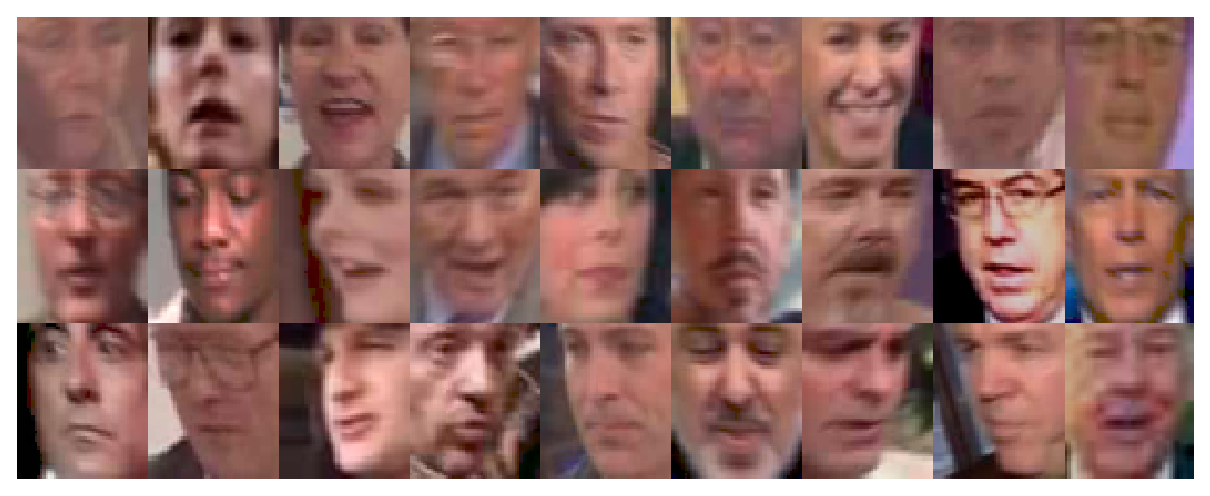
\includegraphics[width=\linewidth]{Chapters/facev1/Fig7.eps}
    \caption{Examples of degraded images produced using a predefined procedure from \citep{SohnLZY0C17}. See \tab{comparison_other} for comparison with our augmentation. }\label{fig:predefined}
  \end{figure}
  
The results for training on the YTF dataset with  method \citep{ganin2016domain} are shown in \tab{comparison_other}: 
model A corresponds to our \textit{ft union} model, model B combines the image-level domain-adaptation (the same as for \textit{ft union}) and feature-level domain adaptation, model C uses feature-level domain adaptation only. Feature-level domain adaptation improves the performance slightly if combined with the image-level domain adaptation (model B compared to model A), whereas applied alone, it leads to overfitting (model C).

We have also compared our approach to the method described in \citep{SohnLZY0C17}. It aims at performing feature-level adaptation and restoration using artificially-degraded data as a bridge between the two domains. The goal is to train such a model that would be tolerant to image degradation and at the same time, retain the representations of the source domain data. 
The authors also incorporate a feature-level adversarial loss, and we use that of \citep{ganin2016domain} for our implementation of \citep{SohnLZY0C17} for better comparability. Instead of the Image Classification loss used in \citep{SohnLZY0C17}, we use the BinDev loss as for the other experiments in this work.
Two other losses that were used in \citep{SohnLZY0C17}, apart for Image Classification loss and Domain-Adversarial loss, are Feature Matching and Feature Restoration losses. To implement the scheme from \citep{SohnLZY0C17}, we added these two losses to the final objective function. Additionally, it should be noted that in \citep{SohnLZY0C17}, the network is initialised by the weights of the model trained on the source domain (\textit{ft initial} in our case). We also used the predefined degradation procedure described in \citep{SohnLZY0C17} to generate augmentation data.
%todo insert a picture with examples

The results of our implementation of the scheme from \citep{SohnLZY0C17} are shown in \tab{comparison_other} in rows D-J. All the models D-J are fine-tuned with additional losses from \citep{SohnLZY0C17} (with changes discussed above) starting at the state of \textit{ft inital}. Models D and I differ in the utilized augmentation method. Model I uses pre-defined augmentation procedure ('predefined', see \fig{predefined} for examples) from \citep{SohnLZY0C17}, whereas our CycleGAN-based augmentation is used for D.  We can see that our augmentation results in better performance in comparison to that of \citep{SohnLZY0C17} for our data. We also compared the two augmentation methods for our training scheme \textit{ft-union} and observed very similar results (not shown here).
 To ensure the sanity of our implementation of \citep{SohnLZY0C17}, we also show the role of different subsets of losses in the rows D-H of \tab{comparison_other}. Indeed, we can see that model D, that is trained with the full set of losses, outperforms other models E-H. 

Finally, we can see from \tab{comparison_other}, that our approach (models A and B) outperforms the scheme from \citep{SohnLZY0C17} (model I), and as it can be seen from the comparison, the difference mostly comes from the augmentation method: model D is trained using our CycleGAN-based augmentation and the resulting performance is close to that of our model B.
 


% \subsection{Comparison to feature-level domain adaptation}
% \label{sect:grl}
% We have additionally compared our image-level domain adaptation (all the experiments and discussions above) to the feature-level domain-adversarial adaptation approach~\citep{ganin2016domain}. Tuning this approach required some effort (several modifications from the settings of~\citep{ganin2016domain} were needed to make such adaptation work). We thus built a DANN (Deep Adversarial Neural Network) based on the VGG-face network. The  domain classifier consists of three fully-connected layers: $512$ units in the first two layers (Leaky ReLU \citep{HeZRS15} non-linearities were used) and one classification layer with $1$ unit. Dropout with $0.5$ probability was inserted before the classification layer. The Gradient Reversal layer is attached after the \textit{fc6} layer of VGG-face. We found that schedule for the adaptation parameter  $\lambda$ is very important for this task. Instead of the schedule suggested in \citep{ganin2016domain} (which did not lead to good results in our comparison), we set $\lambda$ to $1e-3$ for the first $20$ epochs and then increased it to $1e-2$. 

% Using the scheme described above when training on the VGG Face dataset, we have achieved the following results: $100$\% - EER was $88.64$, ROC AUC was $96.69$ and the average precision was $52.11$. This is better than the results of our \textit{ft initial} setting, but worse than those of \textit{ft degraded} and \textit{ft union} settings (for the last, the results are $91.31$, $97.80$ and $54.89$ correspondingly). Other setting for feature-level domain adaptation that we have tried lead to worse results.






  
  
  
  
